\footnotesize
% 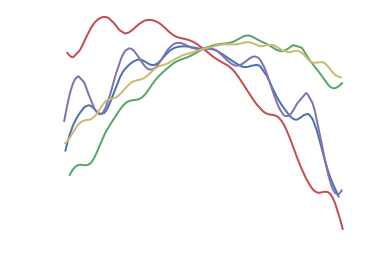
\includegraphics[width=.33\textwidth]{figs/gpSamples/main.png}
\begin{tabular}{cccccc}
\multicolumn{6}{c}{ 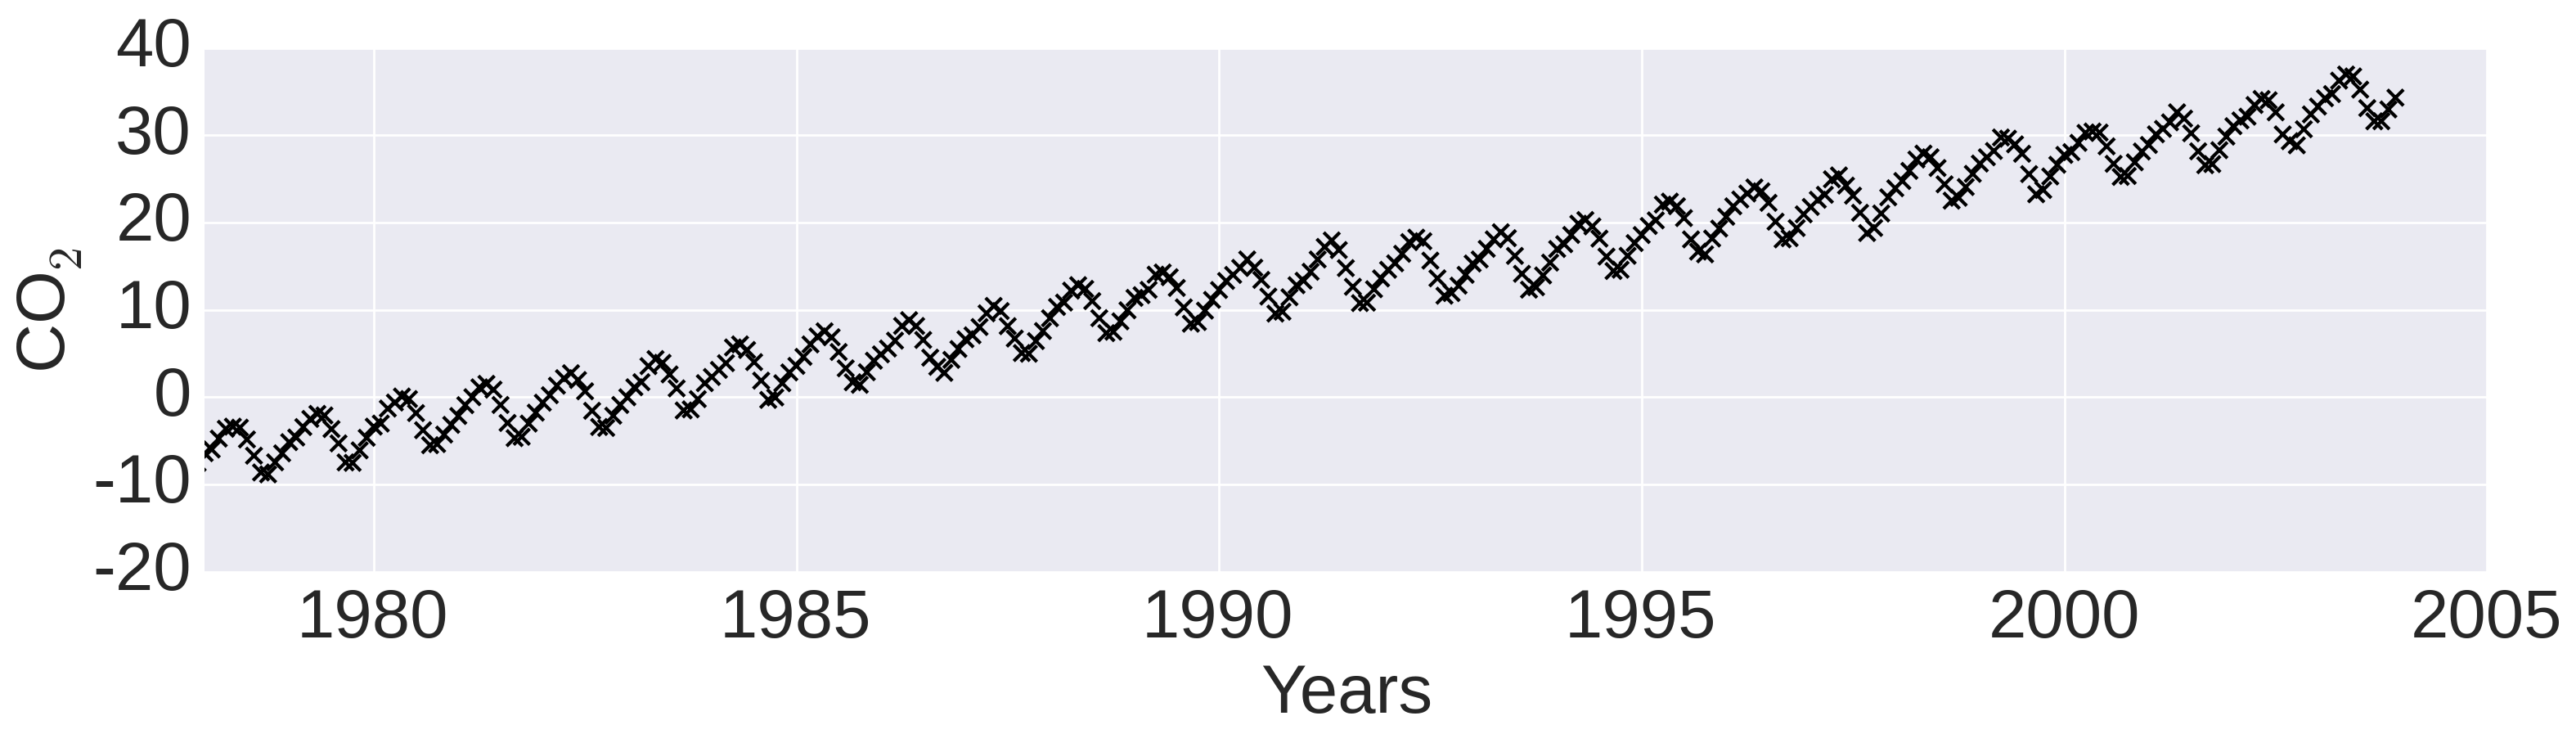
\includegraphics[width=0.8\textwidth]{figs/mauna_data.png}}     \\                                               
\multicolumn{6}{c}{\tikzmark{a}}     \\  
\multicolumn{6}{c}{}     \\   
\multicolumn{6}{c}{\tikzmark{b}}     \\  
\multicolumn{6}{c}{ 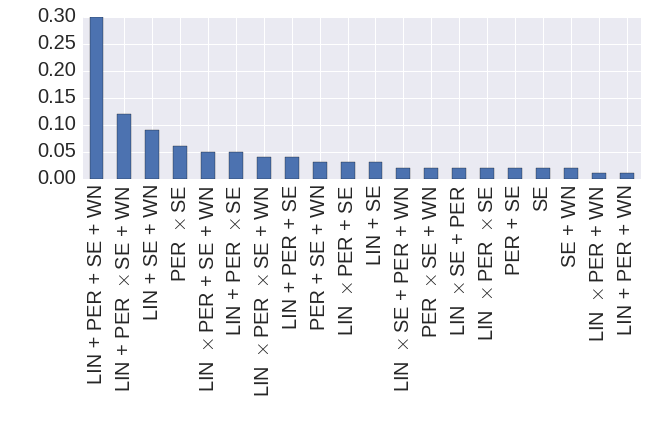
\includegraphics[width=0.6\textwidth]{figs/mauna_structure.png}}     \\                                               
\multicolumn{6}{c}{\tikzmark{c}}     \\  
\multicolumn{6}{c}{}     \\   
\multicolumn{6}{c}{\tikzmark{d}}     \\           
\multicolumn{6}{c}{\normalsize \color{blue} What is the probability of a trend, a recurring pattern {\bf and} noise in the data?}     \\               
\multicolumn{6}{c}{$P\big((\text{LIN}\lor\text{LIN}\times\text{SE})\land
(\text{PER}\lor\text{PER}\times\text{SE}\lor\text{PER}\times\text{LIN})\land
(\text{WN}\lor\text{LIN}\times\text{WN})\big)
$}                                                     \\
          &      \tikzmark{trend_part}     &  &    \tikzmark{recurring_part}   &     \tikzmark{noise_part}     &                          \\
          &          &  &  &  &                            \\
\multicolumn{2}{c}{\tikzmark{trend}}& & &   \multicolumn{2}{c}{ \tikzmark{noise}} \\  
\multicolumn{2}{c}{\normalsize \color{blue} Is there a trend?}& & &   \multicolumn{2}{c}{ \normalsize \color{blue} Is there noise?} \\
\multicolumn{2}{c}{$P(\text{LIN}\lor\text{LIN}\times\text{SE})$}& & &   \multicolumn{2}{c}{$P(\text{WN}\lor\text{LIN}\times\text{WN})$} \\
\multicolumn{2}{c}{\tikzmark{trend_below}}& & &   \multicolumn{2}{c}{ \tikzmark{noise_below}} \\  

        &          &  &       &       &                            \\
         \tikzmark{lin}  &\tikzmark{linse}             &         &       &                 \tikzmark{linwn}  &\tikzmark{wn}            \\

           {\normalsize \color{blue} A linear trend?}  &{\normalsize \color{blue} A smooth trend?}   &         &       &                 {\normalsize \color{blue} Heteroskedastic noise?}  &{\normalsize \color{blue} White noise?}           \\
          $P(\text{LIN})$& $P(\text{LIN}\times\text{SE})$         &          &    &$P(\text{LIN}\times\text{WN})$  &$P(\text{WN})$    \\
         &          &         &       &                &          \\
         &          &         &\tikzmark{recurring}       &                &          \\
      \multicolumn{6}{c}{\normalsize \color{blue} Is there repeating structure?} \\
  \multicolumn{6}{c}{$P(\text{PER}\lor\text{PER}\times\text{SE}\lor\text{PER}\times\text{LIN})$} \\
     & &    \multicolumn{2}{c}{\tikzmark{recurring_below}} & &\\
      &          &  &       &       &                            \\
         &  \tikzmark{per}        &   \multicolumn{2}{c}{\tikzmark{perse}}     &   \tikzmark{perlin}    &    \\
        \multicolumn{2}{c}{$P(\text{PER})$}         &           \multicolumn{2}{c}{$P(\text{PER}\times\text{SE})$}         &                   \multicolumn{2}{c}{$P(\text{PER}\times\text{LIN})$}           \\
   &          &  &       &       &                            \\
        \end{tabular}
 \begin{tikzpicture}[overlay, remember picture, yshift=.25\baselineskip, shorten >=.5pt, shorten <=.5pt]
   \draw [->] ({pic cs:a}) to ({pic cs:b});
      \draw [->] ({pic cs:c}) to ({pic cs:d});
    \draw [->] ({pic cs:recurring_part}) to ({pic cs:recurring});
    
     \draw [->] ({pic cs:recurring_below}) to ({pic cs:per});
      \draw [->] ({pic cs:recurring_below}) to ({pic cs:perse});
     \draw [->] ({pic cs:recurring_below}) to ({pic cs:perlin});
    
    
      \draw [->] ({pic cs:trend_part}) to ({pic cs:trend});
        \draw [->] ({pic cs:trend_below}) to ({pic cs:lin});
    \draw [->] ({pic cs:trend_below}) to ({pic cs:linse});
    
     \draw [->] ({pic cs:noise_part}) to ({pic cs:noise});
       \draw [->] ({pic cs:noise_below}) to ({pic cs:wn});
         \draw [->] ({pic cs:noise_below}) to ({pic cs:linwn});
  \end{tikzpicture}
%  \multicolumn{3}{c}{$P(\text{PER}\lor\text{PER}\times\text{SE}\lor\text{PER}\times\text{LIN})$}